%Inserite il titolo del documento
\newcommand{\titolo}{Relazione di Intelligenza Artificiale}
%Inserite la prima data di creazione del documento
\newcommand{\datacreazione}{12 settembre 2014}
%Inserite la versione attuale del documento
\newcommand{\versione}{1.0}

\newcommand{\gl}{\textsuperscript{[g]}}

%%This is a very basic article template.
%%There is just one section and two subsections.
\documentclass[11pt,a4paper,italian]{extarticle}
\usepackage[italian]{babel}
\usepackage[utf8x]{inputenc}
\usepackage{graphicx}%per usare le immagini
\usepackage{amsmath}
\usepackage{amsfonts}
\usepackage{amssymb}
\usepackage{color}
\usepackage{hyperref}
\usepackage[all]{hypcap}
\usepackage{ifthen}
\usepackage{wrapfig}
\usepackage{indentfirst}
\usepackage{fancyhdr} %pacchetto per le intestazioni
\pagestyle{fancy} %uso del pacchetto
\usepackage{float}
\usepackage{pdflscape}
\usepackage{subfigure}

\fancyhead{} %annulla head di default
\fancyfoot{} %annulla foot di default
\usepackage{lastpage} %setto pg di pgtot a rfoot
\usepackage{booktabs}%pacchetto per tabelle nuove
\usepackage{eurosym} %per avere simbolo euro
\usepackage{multirow}%per avere celle su piu righe


\usepackage[top=2cm,bottom=4cm,left=80pt,right=80pt]{geometry} %disegna la linea
\setlength{\headheight}{2cm} %settato grandezza header

\rfoot{pagina \thepage\ di \pageref{LastPage}}
\lfoot{Versione: \versione} %setto versione doc a lfoot

\renewcommand{\footrulewidth}{1.5pt} %ridefinisco il valore della riga di intestazione
\renewcommand{\headrulewidth}{1.5pt} %ridefinisco il valore della riga di pie' di pagina
\addtolength{\headwidth}{\marginparsep}
\addtolength{\headwidth}{\marginparwidth}


\hypersetup
{
	colorlinks=true,
	linkcolor=blue,
	urlcolor=blue
}

\cfoot{
	\titolo \\ 
}


\newenvironment{infodocumento}{%
	\begin{center}%
		\begin{tabular}{r|l}%
            \multicolumn{2}{c}{\large{\textbf{Informazioni sul documento}}}\\%
			\hline%
			
}%
{
		\multirow{2}{*}{Distribuzione} & Alessandro Zonta, il tutor aziendale \\& e il tutor interno.
		\end{tabular}%
	\end{center}%
}

\newboolean{redarre}
\newboolean{approvare}
\newboolean{verificare}
\newboolean{distribuire}
\setboolean{redarre}{true}
\setboolean{approvare}{true}
\setboolean{verificare}{true}
\setboolean{distribuire}{true}
\newcommand{\Nome}[1]{\textbf{Nome}&#1\\}
\newcommand{\Creazione}{\textbf{Data di creazione}&\datacreazione\\}
\newcommand{\Versione}{\textbf{Versione}&\versione\\}
\newcommand{\UltimaModifica}{\textbf{Data di ultima modifica}&\today\\}
\newcommand{\Formale}{\textbf{Stato}&Formale\\}
\newcommand{\Preliminare}{\textbf{Stato}&Preliminare\\}
\newcommand{\Esterno}{\textbf{Uso}&Esterno\\}
\newcommand{\Interno}{\textbf{Uso}&Interno\\}


\newcommand{\Reda}[1]{\hline \textbf{Redazione}&\parbox{0.65\textwidth}{#1}\\}

\newcommand{\Ver}[1] {\hline \textbf{Verificatore}&\parbox{0.65\textwidth}{#1}\\}

\newcommand{\App}[1] {\hline \textbf{Approvazione}&\parbox{0.65\textwidth}{#1}\\}
  



\newenvironment{regmodifiche}{%
	\vspace{60px}
	\begin{Large}
    	\textbf{Registro delle modifiche}\\\\%
	 \end{Large}\\
	 \begin{tabular}{|c|c|c|}%
    	\hline
    	\parbox{0.25\textwidth}{Data \& Autore} & 
    	\parbox{0.1\textwidth}{Versione} & 
    	\parbox{0.57\textwidth}{Modifiche}\\
    	\hline
 	\end{tabular}
}%

\newcommand{\modifica}[4]{
		\begin{tabular}{|c|c|c|}%
			\parbox{0.25\textwidth}{\ \\ #1 \\ #3\\} & 
			\parbox{0.1\textwidth}{#2} & 
			\parbox{0.57\textwidth}{#4}\\ 
			\hline
		\end{tabular}%
}

%importo package per includere porzioni di codice
\usepackage{lmodern}
\usepackage{listings}
\usepackage[labelformat=empty]{caption}
\newenvironment{gigante}[1]{
	\fontsize{30mm}{5mm}\selectfont
	\selectfont	\textbf{{#1}}
	\normalfont
}

\begin{document}

%INIZIO PRIMA PAGINA NON MODIFICARE
\begin{titlepage}


\vspace{60pt}

\begin{center} 
		\vspace{10pt}
		\fontsize{10mm}{12mm}\selectfont Università degli Studi di Padova\\
		\fontsize{8mm}{10mm}\selectfont Dipartimento di Matematica\\
		Corso di Informatica Magistrale
\end{center}
\vspace{30pt}
\begin{center} 
		\fontsize{10mm}{12mm}\selectfont \textbf{Intelligenza Artificiale}\\
		\fontsize{8mm}{10mm}\selectfont Realizzazione di un player per il gioco di carte UNO
\end{center}
\vspace{100pt}
\begin{center}
	\fontsize{5mm}{7mm}\selectfont\textbf{Studente:} Giacomo Quadrio\\
	\fontsize{5mm}{7mm}\selectfont\textbf{Matricola:} 1061566\\
	\vspace{5pt}
	\fontsize{5mm}{7mm}\selectfont\textbf{Studente:} Alessandro Zonta\\
	\fontsize{5mm}{7mm}\selectfont\textbf{Matricola:} 1081173
\end{center}
\vspace{5pt}
\vspace{5pt}
\begin{center}
	\fontsize{5mm}{7mm}\selectfont A.A. 2013/2014
\end{center}
\end{titlepage}
%FINE PRIMA PAGINA

\tableofcontents

\newpage
\section{Introduzione}
	Nel seguente documento verrà presentato il progetto per il corso di Intelligenza Artificiale svolto dagli studenti Quadrio Giacomo e Zonta Alessandro.  Il progetto consiste nella realizzazione di un player per il gioco di carte UNO attraverso l’applicazione degli algoritmi di ricerca con avversari visti a lezione.
\newpage

\section{Ricerca con avversari}
	La ricerca con avversari rientra nella tipologia degli algoritmi di intelligenza artificiale che prevede un ambiente multiagente, ovvero più agenti operano all’interno dello stesso ambiente ed ognuno deve considerare, per le sue azioni, quelle degli altri. Nel progetto gli agenti che operano sono due, Min e Max, il gioco risulta essere a somma zero, ovvero il payoff totale è lo stesso per ogni istanza del gioco, e si costruirà un albero di gioco per decidere come procedere nell’analisi. Scendendo nel dettaglio abbiamo che innanzitutto non dobbiamo trovare la strategia ottima per arrivare all’obiettivo ma dobbiamo scegliere la mossa che conduce alla posizione con valore MinMax più alto ovvero la mossa che ci da il miglior vantaggio sul nostro avversario, che assumiamo giochi in maniera ottima. 
\newpage

\section{Il Gioco di carte UNO}
	UNO è un gioco di carte statunitense creato nel 1971. Il numero dei giocatori può variare da 2 a 10. 
	\begin{figure}[h]
		\centering
		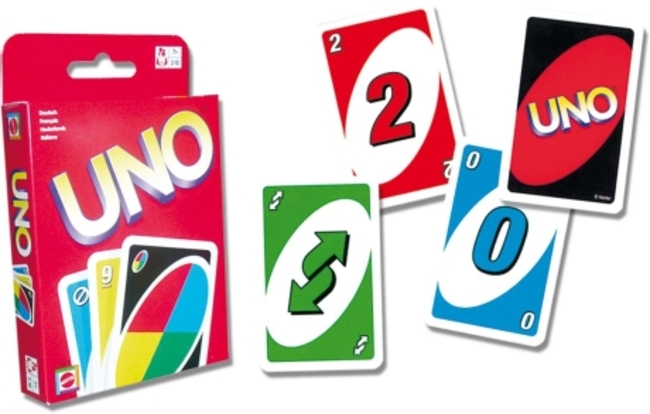
\includegraphics[scale=1]{uno.jpg}
		\caption{Gioco UNO}
		\label{fig0}
	\end{figure}
	
		\subsection{Le carte}
			All'interno di una confezione di gioco sono contenute carte così distribuite:
			\begin{itemize}
			\item 19 carte di colore \textit{Rosso} che vanno dall'1 al 9 (2 serie) più uno 0
			\item 19 carte di colore \textit{Blu} che vanno dall'1 al 9 (2 serie) più uno 0
			\item 19 carte di colore \textit{Giallo}  che vanno dall'1 al 9 (2 serie) più uno 0
			\item 19 carte di colore \textit{Verde}  che vanno dall'1 al 9 (2 serie) più uno 0
			\item 8 carte \textit{Pesca Due} dei vari colori sopracitati
			\item 8 carte \textit{Cambio giro} 
			\item 8 carte \textit{Salta} o \textit{Stop} sempre dei colori sopracitati
			\item 4 carte \textit{Jolly} o \textit{Cambio colore}
			\item 4 carte \textit{Jolly Pesca Quattro} o \textit{Cambio colore - Pesca quattro} non valente per iniziare il gioco
			\end{itemize}
			per un totale di 108 carte.
			
		\subsection{Obiettivo del gioco}	
			Colui che riesce a esaurire tutte le carte che ha nella sua mano vince la partita.
			
		\subsection{Procediemnto del Gioco}
			Il sorteggio del mazziere avviene mediante pesca di una carta dal mazzo; colui che pesca quella con il numero più alto, diviene il mazziere.	\\
			Dopo l'estrazione del mazziere, le carte vengono rimescolate e distribuite 7 a testa. La porzione di mazzo rimanente, detta "mazzo pesca", viene posata sul tavolo a dorso coperto, e la prima viene girata, andando così a formare il cosiddetto "mazzo scarti".\\
			Il giocatore alla sinistra del mazziere comincia il gioco (procedendo il giro in senso orario): questi deve scartare una carta dalle proprie a disposizione, compatibile con quella in cima al mazzo scarti per colore o per numero. Ciò significa che la carta deve avere colore o numero uguale alla prima carta sul banco: ad esempio, se la carta sul banco è un 7 rosso, il giocatore può scartare una carta numerata di colore rosso, o volutamente un 7 di qualsiasi colore; da allora il colore può cambiare e così via. Alternativamente, il giocatore può usare una carta Azione (le carte azione colorate devono essere compatibili con la carta del mazzo scarti). Non si può scartare più di una carta per turno.\\
			Se il giocatore non ha a disposizione carte da scartare, ha l'obbligo di pescarne una dal mazzo pesca. Il giocatore ha l'obbligo di tirare una carta in suo possesso, se compatibile con quella che si trova sul mazzo scarti. \\
			Quando un giocatore scarta una delle sue due carte rimaste così rimanendo con una sola carta in mano, deve pronunciare "UNO!". La pronuncia della parola deve avvenire prima che la penultima carta che questi gioca raggiunga il mazzo scarti e deve essere detta comprensibilmente.\\
			Una volta che uno dei giocatori seduti al tavolo non ha più carte, si procede al calcolo del punteggio che questi ha conseguito. Nel caso in cui l'ultima carta da giocare sia un pesca 2 o un pesca 4 il giocatore seguente deve comunque prendere il numero di carte corrispondenti.
		
		\subsection{Funzione delle carte Azione}
			Le funzioni delle carte "Azione" sono le seguenti:
			\begin{itemize}
			\item	Carta Inverti o Cambia salto: inverte il senso di gioco da orario ad antiorario o viceversa.
			\item	Carta Salto o Salta turno o Stop: fa saltare un turno al giocatore successivo nel senso del gioco.
			\item	Carta Pesca due carte: il giocatore successivo nel senso del gioco pesca due carte e salta il turno.
			\item	Carta Jolly o Cambio colore: permette al giocatore di scegliere uno tra i quattro colori disponibili (Rosso, Verde, Blu, Giallo).
			\item	Carta Jolly Pesca quattro o Pesca quattro carte: è la carta più potente del gioco. Costringe il giocatore successivo nel senso del gioco a pescare quattro carte ed a saltare il turno. La carta in questione consente, inoltre, a chi l'ha giocata di cambiare il colore del gioco.
			\end{itemize}
			
		\subsection{Implementazione}	
			Abbiamo scelto di implementare il gioco in Java con due modalità: Umano vs CPU o CPU vs CPU. Abbiamo deciso di non implmentare il rimescolamento del mazzo una volta che è finito e di decidere la vittoria in base al giocatore con meno carte in mano. In caso di parità viene assegnata la parità, non è stato implementato un sistema di conteggio dei punti. Una volta che si pesca un acarta dal mazzo automaticamente si passa il turno e anche l'uso della carta Jolly. L'uso della carta Cambio Colore ha gli stessi vincoli della carta Pesca quattro; per essere giocata necessita che in mano non ci siano carte con lo stesso colore di quella sul mazzo scoperto.
			
\section{La scelta della libreria Swing}
	Per il progetto di intelligenza artificiale è stato utilizzato il framework Java denominato Swing per la realizzazione dell'interfaccia grafica. La scelta di utilizzare Swing è derivata dal fatto che queste librerie permettono di creare interfacce grafiche indipendentemente dalla piattaforma su cui viene eseguito il programma finale. Inoltre le diverse parti di essa sono basate su determinate interfacce collegate in modo da consentire facilmente l'aggancio di implementazioni differenti di tali interfacce. Il programmatore può quindi creare un’implementazione personalizzata oppure affidarsi alle versioni di default. 
	Un altro vantaggio della libreria Swing è la sua leggerezza: essa infatti non richiede di utilizzare i controlli della GUI del sistema operativo nativi, poiché disegna i suoi controlli tramite l'uso delle API 2D di Java. Infine, un componente Swing non deve avere per forza un corrispettivo nell'insieme dei componenti nativi del sistema operativo, ciò significa che è possibile realizzare componenti con libertà, sfruttando tutte le risorse messe a disposizione dalle librerie grafiche Java 2D. 
	Leggerezza dell'interfaccia, facilità di utilizzo, portabilità sono le caratteristiche che in definitiva ci hanno spinto ad utilizzare Swing per il nostro progetto di intelligenza artificiale. 
	
	\subsection{Struttura grafica dell'applicazione}
		Per l'applicazione “UNO” abbiamo utilizzato una struttura grafica molto semplice, basata su di una singola finestra che, a seconda delle esigenze, mostra differenti pulsanti e informazioni per poter procedere con l'esecuzione del gioco. 
		
		\begin{figure}[h]
			\centering
			
\includegraphics[scale=1]{1.png}
			\caption{Schermata di selezione del gioco}
			\label{fig1}
		\end{figure}
		
		Nella prima schermata è possibile selezionare due differenti tipologie di gioco, partita CPU contro giocatore umano e partita CPU contro CPU. Dopo aver effettuato la scelta si può dar inizio ad una partita selezionando il pulsante “Inizia gioco”. 
		
		\begin{figure}[h]
			\centering
			
\includegraphics[scale=0.6]{2.png}
			\caption{Quadrato magico inizializzato}
			\label{fig2}
		\end{figure}
		
		Avviato il gioco, la schermata successiva che ci verrà presentata è il tafolo di gioco con presenti su schermo le carte dei due giocatori. Abbiamo deciso di mostrare le carte scoperte di entrambi i player così da offrire una migliore rappresentazione grafica della partita in corso, i due giocatori però non saranno a conoscenza di che carte ha in mano l’avversario. Il gioco è stato quindi inizializzato ed è pronto per essere avviato. Nel caso di un giocatore umano le azioni disponibili saranno quelle visualizzate nell’immagine ovvero ci potrà passare, dichiarare UNO, ricominciare una partita, pescare una carta o selezionare una delle carte che si hanno in mano per poterla lanciare. Se la carta che si seleziona non è compatibile con la carta sulla cima della pila verrà segnalato un messaggio d’errore.
		
		\subsubsection{Principali informazioni sul codice della componente grafica}
			Per la realizzazione vera e propria dell'interfaccia grafica si è utilizzato un Frame principale, nel quale venivano di volta in volta modificati i contenuti a seconda delle esigenze. Nel dettaglio si è creata una classe FrameP che estende la classe base Jframe : \textit{class FrameP extends Jframe}\\\\
			
			In questa classe sono stati innanzitutto inizializzati tutti i vari componenti che verranno utilizzati nelle varie maschere e che saranno disegnati, aggiornati o spostati dalle varie funzioni a seconda dello stato in cui si trova il gioco. \\\\
			
			Per il layout generale della finestra si sono utilizzati principalmente tre tipologie di layout: BoxLayout, FlowLayout e BorderLayout. Per poter realizzare schermate più complesse si è inoltre scelto di adottare la tecnica dei layout innestati, di conseguenza si sono inseriti nel container principale altri container, creando quindi una struttura che ci permettesse una gestione più semplice degli elementi presenti a schermo. \\\\
			
			Qui di seguito sono elencati brevemente i tre layout in questione: 
			\begin{itemize}
				\item \textbf{BoxLayout} Permette di inserire gli elementi l’uno di seguito all’altro. Nel dettaglio abbiamo utilizzato una struttura a pila verticale nella quale si aggiungevano di volta in volta gli oggetti grafici uno sotto all’altro. Questo layout è risultato essere molto comodo per la gestione del tavolo di gioco.
				\item \textbf{FlowLayout} Si tratta della tipologia di layout più semplice in quanto con esso si inseriscono gli elementi orizzontalmente uno di fianco all’altro. E’ stato utilizzato per mostrare le carte che i giocatori hanno in mano.
				\item \textbf{BorderLayout} Questo layout è molto particolare in quanto suddivide la finestra in cinque differenti zone salienti. La zona NORD per la parte alta, la zona EAST per la parte centrale destra, la zona WEST per la parte centrale sinistra, la zona CENTER per la parte centrale e la zona SOUTH per la zona bassa. Esso è stato utilizzato per la schermata principale e le varie schermate di transizione tra un’azione e l’altra del giocatore. Di seguito potete vedere un esempio della struttura del BorderLayout.
			\end{itemize}
			
			\begin{figure}[h]
				\centering
				
\includegraphics[scale=0.6]{3.png}
				\caption{le aree di BorderLayout}
				\label{fig3}
			\end{figure}
				
	\subsection{Gestione degli eventi}
		La gestione degli eventi, infine, è stata realizzata utilizzando le librerie AWT (Abstract Window Toolkit), per la precisione il package relativo alla gestione degli eventi denominato awt.event. 
\begin{lstlisting}
...

start.addActionListener(new StartGame());

...

class StartGame implements ActionListener {
		
  public void actionPerformed(ActionEvent e){
	
    JButton button = (JButton)e.getSource();
    if(button.getText()=="Inizia gioco"){
	  if(game_1.isSelected()){
		InsertName();
		start.removeActionListener(this);
	  }else{
		
			if(game_2.isSelected()){
				GameTable();
				start.removeActionListener(this);
			
			}
		
		}
    }
	
  }

}

\end{lstlisting}

		Al bottone adibito all'azione è stato aggiunto un ascoltatore per rilevarne la pressione. Una volta eseguita l'azione viene richiamata l'apposita classe che ne contiene le operazioni da eseguire. A seconda del tasto premuto l'azione eseguita sarà differente e ciò permette di poter accedere alle varie funzionalità del gioco “UNO”. Gli ascoltatori sono stati utilizzati per poter permettere varie azioni all’interno del gioco come l’avvio di una partita, la selezione della carta da giocare, il riavvio della partita ecc.
		
		
		
\section{Gestione Logica}		
	Per lo sviluppo degli algoritmi scelti e del gioco in se sono state pensate cinque classi principali che racchiudono tutta la logica del programma. Essendo il gioco UNO un gioco di carte si è pensato a una classe che implementa la singola carta e le informazioni che si porta dietro ed a una classe che implementa il mazzo di carte con la relativa gestione. Una classe gestisce il gioco implementando le operazioni per farlo iniziare e finire e due classi, una che deriva dall'altra, che implementano il giocatore umano e quello controllato dal pc. Questo serve perchè il gioco implementa la sfida tra umano contro CPU e CPU contro CPU.
	
	\subsection{Carta}
		Questa è la classe che implementa le caratteristiche di una carta di UNO. Basilari per il gioco sono il colore della carta (il gioco UNO ne prevede 4: rosso, giallo, verde e blu) e il valore della carta. Le carte vanno dallo 0 al 9 e ne esistono alcune speciali come il ``pesca due carte'',``pesca quattro carte e cambia colore'' ,``cambia colore'' ,``stop'' e ``inverti il giro''. Un'alta proprietà importante è la propietà valore che verrà assegnata dall'algoritmo Minimax o Potatura $\alpha$-$\beta$ e che ci permetterà di capire quale è la carta migliore da giocare. Infine possiede due proprietà utili per gli algoritmi citati sopra, cioè se causa il salto del turno dell'avversario e se è stata ``usata''. Oltre ai normali getter e setter e ai costruttori questa classe non contiene nulla di più.
		
	\subsection{Mazzo}
		Questa classe implementa le caratteristiche del Mazzo del gioco. Troviamo due liste le quali conterranno una tutte le carte presenti nel mazzo coperto e l'altra il mazzo delle carte scartate. È presente un metodo che permette di mescolare le carte del mazzo. Questo metodo utilizza la funzionalità \textit{shuffle} integrata in Java. Sono presenti i metodi per pescare una carta dal mazzo coperto, per restituire la prima carta del mazzo scarti, per scegliere a caso la prima carta scartata all'inizio della partita, per buttare una carta nel mazzo scarti e due metodi utili per clonare il mazzo e resettarlo ai valori dati per parametro. Questi due ultimi metodi sono molto utili quando si ritorna dalla ricorsione per ristabilire i valori presenti nel mazzo prima di aver eseguito a ricorsione.
		
	\subsection{Giocatore}
		Le azioni che il giocatore umano può effettuare sono implementate in questa classe. Sono presenti tre proprietà: il nome del giocatore, la lista delle carte che il giocatore tiene in mano e un riferimento alla classe che gestisce il gioco presente dopo in questa relazione. Grazie a questo riferimento è in grado di poter modificare il mazzo durante il gioco. La clase implementa i metodi per pescare una carta dal mazzo e aggiungerla alla propria lista di carte in mano, per giocare una carta una volta selezionata dalla UI e per compiere le azioni di passare il turno, dichiarare UNO e dichiarare Vittoria. Quando clicco su una carta potrebbe essere che tale carta non sia giocabile, oppure quando tocca al giocatore CPU esso deve controllare se la carta presa in considerazione è giocabile; per questo è stato creato un metodo che dato in ingresso la carta presa in considerazione, la carta sul banco, le carte in mano e l'ultimo colore valido (può essere che sia diverso dalla carta sul banco grazie all'azione di cambia colore o pesca 4 carte) restituisce vero o falso se tale carta è giocabile. È possibile che una carta si agiocabile anche se ha colore diverso ma presenta lo stesso simbolo.
		
	\subsection{GiocatoreCPU}	
		Questa classe si occupa del giocatore controllato dal computer. Dato che è una normale estensione, GiocatoreCPU estende la classe Giocatore così da poter riutilizzare metodi comuni senza riscriverli due o più volte. Qua sono presenti i metodi più importanti del proggetto dato che verte su questi: sono presenti i metodi che implementano il \textbf{Minimax} e la \textbf{Potatura $\alpha$-$\beta$}. Dato che differiscono di molto poco questi due algoritmi è stato deciso di implementarli assieme e distinguere le due scelte tramite una variabile booleana. L'implementazione avviene in tre diversi metodi privati. Il primo inizializza li stati necessari per il corretto funzionamento, avvia l'algoritmo e in base al risultato seleziona la mossa miglire da compiere. Dato che UNO è un gioco di carte, le carte iniziali dell'avversario sono sconosciute. Dalla teoria si sà che tipicamente si può calcolare una probabilità per ogni possibile ordine delle carte quindi si è deciso di ripetere l'algoritmo 50 volte ogni volta con le carte dell'avversario differenti (generate randomicamente ogni volta che viene richiamato l'algoritmo) e di scegliere l'azione che vince più mani in media. All'inizio si era ipotizzato ripetere l'algoritmo per 100 volte ma si è notato che la maggior parte delle volte veniva scelta l'azione ottima al primo colpo quindi si è deciso di scendere a 50 volte per essere sempre sicuri che venga scelta l'azione migliore ma ad una velocità maggiore. \\
		
\begin{lstlisting}
for(int i = 0 ; i < 50; i++){
    //devo anche ipotizzare le carte che ha in mano il mio avversario. 
    //Non conosco ne quante carte ha in mano l'avversario ne quali sono
    //quindi devo
    //generare le carte in mano all'avversario secondo le probabilita'
    //di presenza di quelle carte
    //ipotizzo che in mano abbia esattamente il mio stesso numero di
    //carte
    List<Carta> carteInManoMin = this.GeneraCarteAvversario(
    carteInManoMax.size(), mazzoDaUsare); 
    //se ricordo usata e' true devo controllare che sia sempre 
    //true ad ogni passo
    if(ricordoUsata) carteInTavolaMinimax.get(
    carteInTavolaMinimax.size() -1 ).setUsata(true);
    //eseguo algoritmo minimax. Mi restituisce il valore
    //del ramo da scegliere
    int risultato = this.TurnoDiMax(carteInManoMax, carteInManoMin,
    carteInTavolaMinimax, mazzoDaUsare, -10000, 10000, isMinimax, -1,
    ultimoColoreValido);
    //ottengo index della carta scelta da giocare
    Integer ris = this.CartaSceltaMinimax(carteInManoMax, risultato,
    carteInTavolaMinimax, ultimoColoreValido);
    //se ritorna null devo pescare una carta quindi uso size+1 per
    //tenerlo conto
    if(ris == null){
        vettoreConteggioUsoCarta[carteInManoMax.size()]++;
    }else{
        vettoreConteggioUsoCarta[ris]++;
    }
    //ogni volta devo effettuare il minimax o potatura con il
    //mazzo resettato alla condizione iniziale
    mazzoDaUsare.ResetMazzo(mazzoRESET);
}
\end{lstlisting}
		
		Sul pezzo di codice riportato possiamo notare la chiamata al metodo ``TurnoDiMax'' fondamentale per gli algoritmi scelti. Dato che il \textbf{Minimax} e la \textbf{Potatura $\alpha$-$\beta$} non differiscono molto, sono stati implementati con gli stessi due metodi (``TurnoDiMax'' e ``TurnoDiMin'') e grazie alla variabile booleana \textit{isMinimax} siamo in grado di distinguere quali dei due algoritmi stiamo usando. I parametri passati al metodo sono comuni ai due algorimti tranne per i valori di $\alpha$ e $\beta$ (inizializzati a -10000 e +10000) che sono utilizzati solamente dalla Potatura $\alpha$-$\beta$. Nel codice si può notare anche il metodo che dato il risultato ottenuto dagli algoritmi ci restituisce la carta da giocare ed infine è presente l'incremento all'indice presente su un vettore che conteggia le volte su 50 che quella carta è stata scelta.
		
		\paragraph{TurnoDiMax}
		Implementazione della parte di MAX dell'algoritmo. Riceve in ingresso lo stato del gioco attuale (carte in mano a MAX, carte in mano a MIN, mazzo totale), le due variabili $\alpha$ e $\beta$ necessarie per la potatura, la variabile booleana che distinge se stiamo eseguendo l'algormitmo Minimax o la Potatura $\alpha$-$\beta$, il livello raggiunto nella discesa dell'albero e l'ultimo colore valido di gioco. All'inizio vengono effettuati due controlli: se abbiamo raggiunto una foglia dell'albero o se abbiamo raggiunto il limite deciso dal test di taglio. In entrambi i casi ritorniamo il valore del nodo definito da una funzione di valutazione o dal fatto che il giocatore ha vinto o perso. Successivamente ci sono i controlli sulla carta precendente. Se era una carta Jolly (+4 e cambia colore), una carta +2 o una stop/cambia giro devo agire in conseguenza all'effetto della carta, come pescare carte o saltare il turno. Se quest'utlimo è il caso che si verifica esco direttamente dalla funzione ritornando NULL che verrà interpretato come azione di saltare il giro. Se questi controlli vengono superati allora siamo sicuro che è il nostro turno e posso procedere con la scelta delle carte. Per ogni carta consistente con quella scoperta sul banco devo richiamare TurnoDiMin per ottenere il valore minimax di quel sottoalbero generato dal gioco della carta. Qui entra in campo la variabile booleana che ci permette di usare le due tecniche di ricerca del valore, se stiamo usando il semplice Minimax devo tenermi in memoria il massimo valore restituito da TurnoDiMin; se stiamo usando la Potatura $\alpha$-$\beta$ se trovo un valore che è maggiore di $\beta$ posso restituire quel valore risparmiando la visita di tutti i sottoalberi rimenenti, altrimenti aggiorno solamente $\alpha$.\\
		Ora mostro degli estratti di codice di questo metodo che esprimono in codice quanto appena detto. \\
	
\begin{lstlisting}
//aumento di 1 il livello dell'albero
livello++;
//se questa e' l'ultima azione da fare allora restituisci valore
// funzione obiettivo.
//setto valore funzione obiettivo a +10 quando vince
if(this.TerminatoAlbero(carteInManoMax)){
  return 100;
}
//controllo le carte gioabili perche se sono zero devo passare il
//turno e pescare una carta quindi richiamare il mio avversario
//sulla sua carta giocata
//devo controllare anche se l'ultima carta giocata e' stata un piu'
//due o piu' quattro o salta turno o inverti giro perche' io salto
//il turno e tocca di nuovo all'avversario
Carta ultimaCartaGiocata = carteInTavola.get(carteInTavola.size() -1 );
//se voglio limitare la profondita' ad un livello
//prefissato invece che esplorare il tutto utilizzo questo codice
if(this.TestTaglio(livello)){
  return this.ValutaMossa(ultimaCartaGiocata, carteInManoMax,
    carteInManoMin, true);
}	
.... gestione Jolly (+4,+2,cambia colore,stop,cambia giro)	
//setto counter che mi permettera' di verificare quante cart
//e giocabili avevo in mano
int countNumeroCarteGiocate = 0;
//setto valori ad un numero sicuramente inferiori a tutti 
//quelli possibili che usciranno per usarlo come minimo
int valori = -5000;
for(int i = 0; i < carteInManoMax.size(); i++){
//prima di giocare la carta devo verificare se questa carta e' 
//giocabile. Se la funzione ritorna true allora posso giocare 
//la carta, se la funzione ritorna false non posso
//giocare quella carta.
 if(this.CheckCartaGiocabile(carteInManoMax.get(i), ultimaCartaGiocata, 
   carteInManoMax, ultimoColoreValido)){
   .... gestione stato liste pre ricorsione
//devo creare lo stato da passare a min. Quindi una alla volta gioco
//le carte
   carteInTavola.add(carteInManoMax.get(i));
//la rimuovo da carte in mano
   Carta rimossa = carteInManoMax.remove(i);
//se e' un jolly devo cambiare colore
   if(rimossa.getColore()== "Jolly") ultimoColoreValido =
     this.ScegliColore(this._carteInMano, ultimoColoreValido);
//se la carta giocata ha lo stesso simbolo ma e' di colore
 diverso devo cambiare il colore di gioco
   if(rimossa.getColore() != ultimoColoreValido & rimossa.getTipocarta()
    == ultimaCartaGiocata.getTipocarta()) ultimoColoreValido = rimossa.getColore();
//mi faccio restituire valore funzione obiettivo da min
    int valRestituitoAzioneGiocata = this.TurnoDiMin(carteInManoMin, carteInManoMax, 
    carteInTavola, mazzoCarteTotali, alfa, beta, isMinimax, livello, ultimoColoreValido); 
//assegno valore restituito a carta cosi' alla fine so quale albero prendere
    rimossa.setValore(valRestituitoAzioneGiocata);
..... sistemazione liste stato post ricorsione
//ora devo assegnare a valori il malore massimo tra valori e valRestituitoAzioneGiocata
//in valori e' salvato sempre il valore massimio
    if(valRestituitoAzioneGiocata > valori){
      valori = valRestituitoAzioneGiocata;
    }
//controllo se sto facendo potatura alfa beta o no
    if(!isMinimax){//se e' false sto facendo potatura quindi inserisco codice per potatura
    if(valRestituitoAzioneGiocata >= beta){
      return valRestituitoAzioneGiocata;
  }
//alfa <- max(alfa,v)
    if(valRestituitoAzioneGiocata >= alfa){
      alfa = valRestituitoAzioneGiocata;
    }
}
//conto carte giocate da Max
countNumeroCarteGiocate++;
}
}
//se le carte giocate sono pari a 0 vuol dire che non ho giocato nessuna carta
 perche' non potevo e che quindi mi tocca pescare una carta
if(countNumeroCarteGiocate == 0){
return 0; //non ha senso cercare perche' tanto questa e' l'unica azione disponibile
}
//ritorno valori (valore massimo funzione max)
return valori;	
\end{lstlisting}
	
		\paragraph{TurnoDiMin}
		TurnoDiMin, come dice il nome, implementa la parte di MIN dell'algoritmo. È strutturato esattamente come TurnoDiMax con la differenza che piuttosto di ritornare il massimo valore ritorna il minimo e nel caso della Potatura $\alpha$-$\beta$ se il valore restituito dalla chiamata ricorsiva è minore di $\alpha$ allora posso restituire tale valore non visitando i rimanenti sottoalberi, altrimenti aggiorno $\beta$.
		
		\paragraph{Test di taglio}
		Si è visto che ricercare una soluzione esatta con il Minimax non è fattibile dato numero medio di ramificazioni pari a 24 e massima profondità raggiungibile pari a circa 48. Per questo si è scelto di limitare la profondità di ricerca utilizzando un test di taglio e una funzione di valutazione. È stato scelto un limite di profondità che porta in media la conclusione della partita in tempi rapidi anche se certe mosse richiedono comunue abbastanza tempo per essere ``pensate''. Come funzione di valutazione si è scelto di restituire un valore calcolato da tale formula.\\\\
		
		$ [- (carteInManoIo - carteInManoAvversario)] + (carteGiocabiliIo - carteGiocabiliAvversario) $\\\\
		
		Si è visto che restituisce risultati accettabili nei fini della scelta della carta ottima da giocare. Con carte giocabili si intendono le carte dello stesso colore, dello stesso simbolo o le carte Jolly. 
		
		\paragraph{CheckNumeroCarteAllaFineDelMazzo}
		Se durante il gioco finiscono le carte del mazzo si è deciso di assegnare la vittoria della partita al giocatore con meno carte in mano. È inoltre possibile, solo in questa situazione, che i due giocatori finiscano in parità. In tal caso la partita finisce in parità, si è scelto di non implementare una sorta di calcolo del punteggio.
		
		\paragraph{ScegliColore}
		Durante il gioco è possibile che vengano buttate in campo le carte Jolly. Queste permettono di cambiare il colore delle future carte giocate ma solo se non si possegono più carte dello stesso colore della carta presente in campo. Per restituire il nuovo colore di gioco si è scelto di scrivere un metodo che controlla il colore dominante in mano e sceglie quello per il gioco. Se nessun colore fosse dominante si trovano i due colori dominanti e se ne restituisce uno a caso tra i due. Se non c'è nessun colore dominante si restituisce un colore a caso controllando che non sia lo stesso di quello già in gioco.
	
	\subsection{GiocoUno}
		Questa classe gestisce la gestione dell'intero gioco. Presenta come attributi la lista dei giocatori, il riferimento al mazzo, variabili booleane che controllano se ci sono giocatori umani, la tipologia dell'algoritmo e se il gioco è finito. Tiene traccia del colore attuale in gioco e il riferimento al controller che si occupa di far interagire la grafica con la logica. In questa classe sono presenti i metodi per generare le carte del gioco, per capire chi iniza a giocare, per amministrare la partenza e lo svolgimento del gioco. Inoltre ci sono i metodi che vengono richiamati dal controller quando l'umano interagisce con la grafica per scegliere la carta da giocare o decidere di passare il turno.
		
\section{Controller}
	Questa classe è importantissima per il programma dato che gestisce il collegamento tra la logica e la grafica. Si occupa di richiamare i metodi per aggiornar elo stato della view dopo i cambiamenti introdotti dallo svolgere del gioco come pescare una carta o buttarne una giù. Possiede anche i metodi che avvisano con alert se un giocatore ha vinto o ha dichiarato UNO.

\end{document}